% !TEX root = ./main.tex

\section{Delivery}\label{sec:delivery}

This project is delivered in two stages: \textbf{documenting} and \textbf{pruning}. Documenting and recording in the first stage serves as the preparation for the second stage's pruning work of \images{} ecosystem. The existence of pruning stage is to minimize the impact of large amount of backward incompatible API changes, which means backward compatible PRs can happen at any stage. \par

Concerning the GSoC timeline, documenting stage begins from \date{April 22}\footnote{Although the coding officially begins from \date{May 27}, the author will start this project as soon as he's available.} to \date{June 24} (weeks 1-10), and the pruning stage starts from \date{July 1} to \date{August 26} (weeks 12-22). Week 11 serves as a buffer week. \textsf{Phase 1} evaluates the documenting stage, and \textsf{Phase 2} and \textsf{Final} evaluates the pruning stage.

\subsection{Documenting}\label{subsec:documentation}

\subsubsection*{Stage Expectations}

The primary purpose of this stage is to provide traceable records for the next stage's pruning work. There are three types of records generated in this stage: \textbf{ecosystem documentation}, \textbf{developer manual}, and \textbf{RFCs}. \par

Ecosystem documentation illustrates the scope of image ecosystem and relationships between different relevant packages; it helps users and developers to understand this ecosystem and its fundamental principles quickly. Developer manual consists of the style guide, best practice as well as other related community-operating rules; it gives a documented reference to developers to solve potential conflicts. RFCs with detailed lists of API changes and porting operations are proposed as traceable records for the pruning work in next stage. \par

\subsubsection*{Stage Workflow}

This stage is divided into two periods: \textbf{discussion period} and \textbf{RFC drafting period}. Ideally, this stage ends after the \textsf{Phase 1 Evaluation} with regard to GSoC timeline. However, since a lot of repositories are involved in this project, which makes the timeline hard to be stuck to, the following timeline serves in a flexible way.\par

The discussion period begins from \date{April 22} to \date{June 9} (weeks 1 to 7). In this period the community shares ideas and thoughts on the future of APIs and on best practices.\par

In the beginning of the discussion period, an ecosystem documentation be add to \repoimagesgithubio{} as soon as possible to reach a consensus on the future of \images{}, this consensus shall serve as the fundamental principle to all future discussion and development. Ideally, the current \images{} maintainer, i.e., \timholy, is supposed to participate in.\footnote{In case of maintainer being busy on other work, the author will draft a document based on his understanding and post it to the maintainer to get a feedback.}\par

The RFC drafting period begins from \date{May 27} to \date{June 23} (weeks 6 to 9)\footnote{This doesn't mean RFCs can't be drafted before \date{May 27}.}. Based on previous discussions, one or more RFCs are drafted and discussed in this period. The last week of this stage is used for evaluation, merging, and announcement of RFCs.\par

From weeks 1 to 7, many discussions happen simultaneously in the following way:
{\normalsize
\begin{enumerate}
    \item \textbf{Code Review:} dig into source codes of repositories of images ecosystem to find anything that's likely in need of changing. Other mature \langjulia{} packages, and image-processing libraries in other languages such as \reposcikitimage{} and \matlabimageprocessing{} are references.
    \item \textbf{Issue Open:} open an issue for anything worth a discussion, e.g., legacy codes, misplaced codes, codes with bad practice, and undocumented practices and decisions.
    \item \textbf{Decision Making:} The conventional rules are taken: a decision is made when consensus is reached, otherwise the current maintainer of \images{} make the decision. If a decision can't be made before June 16 (Week 8), it'll be dropped as future work.
    \item \textbf{Record:} all approved, rejected, and future-work proposals are documented in a temporary repository - \repogsoctempdoc{}. Developer manual is drafted to \repoimagesgithubio{} when there are enough decisions made.
\end{enumerate}
}

From weeks 6 to 9, RFC drafting\footnote{A \href{https://github.com/tensorflow/community/blob/master/rfcs/yyyymmdd-rfc-template.md}{RFC Template} is available in the Tensorflow community, and \href{https://github.com/tensorflow/community/blob/master/rfcs/20180827-api-names.md}{20180827-api-names.md} is a good API-renaming RFC example.} happen simultaneously in the following way:
{\normalsize
\begin{enumerate}
    \item \textbf{Code Review:} for each approved proposal, find all involved code pieces, and give a solution to it according to the developer manual. The principle of code review is to rigorously stick to decisions made in the discussion period -- either there's one principle or no principle.
    \item \textbf{RFC Post:} post the draft-version of RFC in \repoimagesgithubio{} as WIP PR.
    \item \textbf{RFC Review:} if there's an issue with any item in the proposed RFC, suspend the related items and go back to the discussion workflow until a decision is made.
    \item \textbf{RFC Approval and Announcement:} After approval of RFCs, they are merged as records and announced to the community via slack and discourse. RFC merging and announcement only happen in the last two weeks in case there are more items to be added.
\end{enumerate}
}
RFC details on how the code base is pruned are described in \cref{subsec:prune}.

\subsubsection*{Stage Evaluation}

Four items are evaluated at the end of this stage, i.e., \textsf{Phase 1 Evaluation}:
{\small
\begin{itemize}
    \item 3/10: activity on issues and discussions
    \item 2/10: ecosystem documentation
    \item 2/10: developer manual
    \item 3/10: RFCs
\end{itemize}
}
A score of 6/10 stands for \textsf{Evaluation Pass}.
% end of subsection

\newpage
\subsection{Pruning Code Base}\label{subsec:prune}
After the RFCs being approved and announced to the community, the pruning stage begins. Ideally, this stage begins from \date{July 1} to \date{August 26} (weeks 12-22).

\subsubsection*{Stage Expectations}

The pruning stage is to clean the code base according to the RFC operation guide. There are three types of pruning work:
{\small
\begin{itemize}
    \item symbol renaming, move, and removal -- backward incompatible
    \item API changes -- backward incompatible
    \item API enhancement -- backward compatible
\end{itemize}
}
For the ease of tracking pruning progress, a project/milestone is set in \repoimages{} to track the progress, and each pruning-related PR/issue will be tagged. \par

\subsubsection*{Stage Workflow}

Challenges during this stage are backward incompatibility and complex package dependencies. This section focus on strategies to address these problems. \par

One strategy of the pruning work is to start from packages with the least dependencies to that with the most dependencies. Using terms from \cref{sec:project}, we start from \sname{core packages} (e.g., \repoimagecore{}), to \sname{application packages} (e.g., \repoimagetransformations{}), and finally to the \sname{user-entrance package}, i.e., \repoimages{}. \sname{New packages} are easy to be handled since they're not officially included in \images{} ecosystem yet. \par

\begin{figure}[htbp]
\caption{Dependency Hierarchy of \images{} Ecosystem}
  \centering
  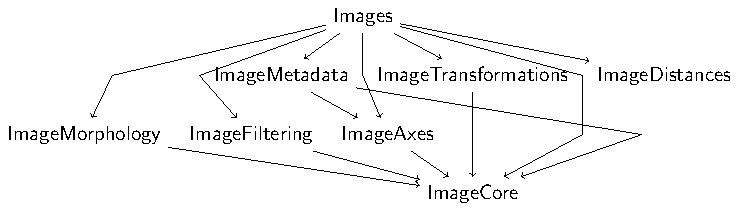
\includegraphics[width=0.8\textwidth]{figures/images_dep.pdf}
\end{figure}

Another strategy is to do all the pruning work in separate branches to reduce the influence brought by its backward incompatibility. In other words, the workflow of pruning work is:
{\normalsize
\begin{enumerate}
    \item create a separate branch \sname{api-prune} in each involved repositories, set up CI environment.
    \item port all methods and symbols in separate branches -- this is backward incompatible
    \item merge each branch into \sname{master}, and tag a minor version to each repository.
    \item freeze minor version for one or two months to let downstream packages upgrade their code base. In the meantime, do backward compatible API enhancement
    \item remove deprecated symbols, methods and their tests, tag a minor version
\end{enumerate}
}
Due to limited time of GSoC, steps 1-3 are counted as a part of GSoC project, and steps 4-5 belong to future work. Since lots of repositories are involved in this project, it's highly possible that this project is still in step 2 when GSoC ends.\par

% \newcommand{\packageA}{package \sname{A}\xspace}
% \newcommand{\packageB}{package \sname{B}\xspace}
% Porting methods from \packageA to \packageB takes the following routine:
% {\normalsize
% \begin{enumerate}
%     \item implement new methods and unit tests in \packageB
%     \item deprecate old methods in \packageA; these codes will be deleted after at least two minor releases.
% \end{enumerate}
% }

\subsubsection*{Stage Evaluation}

With regard to GSoC timeline, this stage includes the \sname{Phase 2} and \sname{Phase final} evaluations. Two attributes can be uses to evaluate the progress: milestone progress (percentage of merged PRs) and absolute number of opened PRs. Both of these are essential to evaluate the success of this project: the former helps evaluate the completeness of this project and the latter helps evaluate the workload and difficulty of this project. Without the latter, one might try to just finish his project without concerning the greater \images{} \version{1.0} progress. \par

The \sname{Phase 2} evaluation shall focus on checking if the pruning work begins as expected. The \sname{Phase final} evaluation shall focus on checking if the major part of pruning work is done.
